\begin{itemize}
\item Etapes de la construction de la courbe ZC.
\item Tableau des parametres
\item Tableau des erreurs de la courbe
\item Figure de la courbe ZC avec points empiriques
\item Figure de la courbe ZC NS et de la courbe forward NS
\end{itemize}

Pour construire la courbe des zéro coupons associée aux taux LIBOR et swap du marché, nous
avons procédé de façon à bien distinguer la courbe zéro coupon de la courbe swap. Pour ce
faire, comme le LIBOR 3 et 6 mois étaient disponibles, nous avons simplement interpolé
avec splines cubiques le swap 9 mois. Puis à partir de cette courbe, par méthode de
bootstrapping tel qu'expliqué par \cite{veronesi} p.~177 nous avons reconstruit
progressivement la courbe zéro coupon. De la même façon, toujours avec un bootstrapping et
une interpolation cubique, nous avons construit successivement une courbe swap interpolée
et la courbe zéro coupon en découlant.

Ensuite, à partir de cette courbe zéro coupon avec des points disponibles à tous les trois
mois, nous avons établi une méthode de moindres carrés avec comme paramètres ceux de la
courbe Nelson Seigel augmentée (voir \cite{diebold}):
\[
  R(0,t) = \beta_0 + \beta_1\left(\frac{1-e^{-t/\theta_1}}{t/\theta_1}\right) +
  \beta_2\left(\frac{1-e^{-t/\theta_1}}{t/\theta_1} - e^{-t/\theta_1}\right) +
  \beta_3\left(\frac{1-e^{-t/\theta_2}}{t/\theta_2} - e^{-t/\theta_2}\right).
\]

Un algorithme à régions de confiance \cite{conn2000trust} a été employé pour déterminer
les paramètres optimaux. Des poids supplémentaires ont aussi été attribués aux premiers
mois ainsi qu'au tout dernier afin de bien répliquer la forme de la courbe impliquée par
les mesures empiriques (voir méthode \verb+load_ns_params():zero.py+ pour plus de
détails).

On obtient alors les paramètres suivants:
\begin{center}
\centering
\begin{tabular}{cccccc}
  \toprule
  $\beta_0$ & $\beta_1$ & $\beta_2$ & $\beta_3$ & $\theta_1$ & $\theta_2$ \\
  \midrule
  \num{0.029376} & \num{-0.029224} & \num{-5.608975} &
                                                       \num{5.565088} & \num{0.564358}
                                                             &
                                                               \num{ 0.560598}\\

\bottomrule
\end{tabular}
\end{center}

On remarque notamment qu'on obtient un taux instantané
$R(0,0) = \beta_0+\beta_1 = \num{0.015148}\%$. Graphiquement, la courbe zéro coupon et le
taux forward instantané sont présentés dans la Figure \ref{fig:ns}.

\begin{figure}
  \centering
  \caption{}
  \label{fig:ns}
  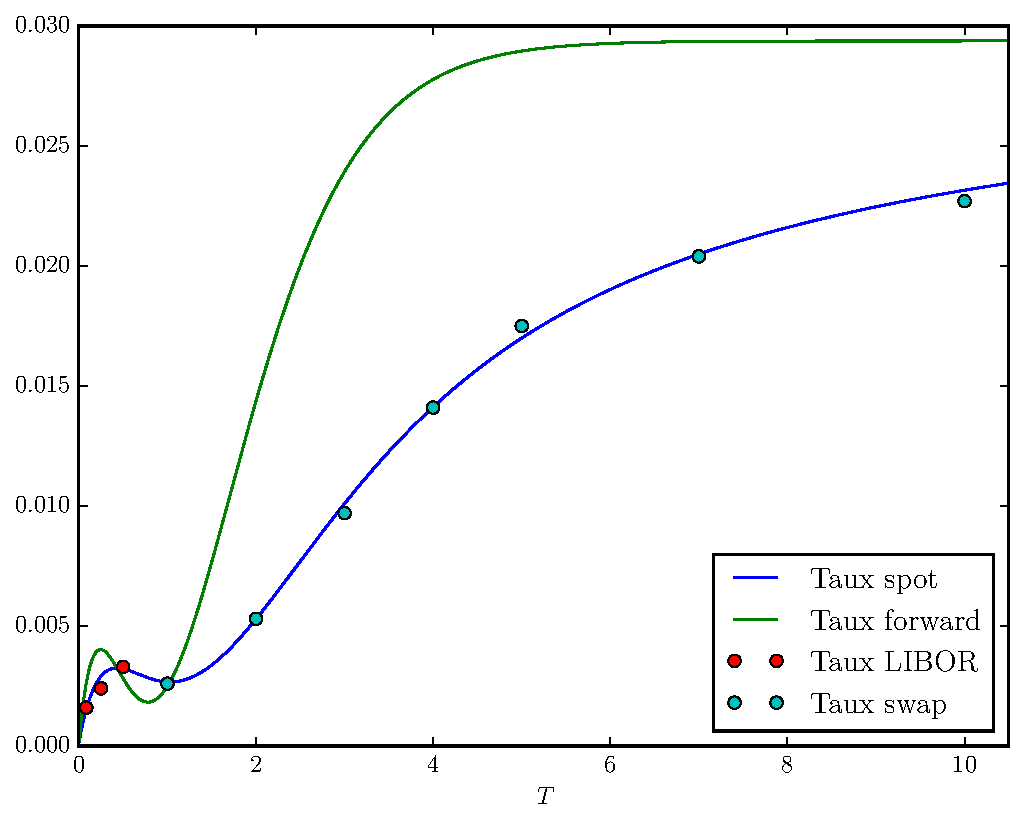
\includegraphics[width=0.3\paperwidth]{../fig/fwd_r.pdf}
\end{figure}



%%% Local Variables:
%%% mode: latex
%%% TeX-master: "rapport"
%%% End:






